\subsection{HTB04 - Friendzone}

    \subsubsection{Escaneo}
        \large{Como primera etapa de la Prueba de Penetración realizamos un escaneo de puertos abiertos en la máquina víctima con la herramienta "Nmap", donde se encuentran siete de ellos.}
        \par
        \begin{figure}[H]
            \centering
            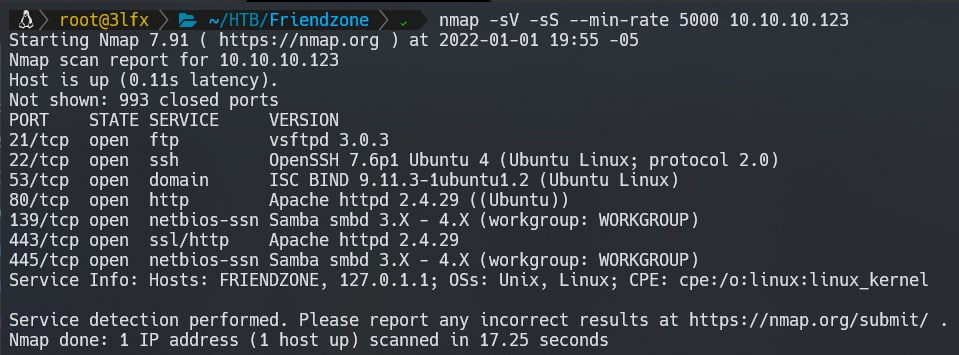
\includegraphics[width=0.99\textwidth]{informe4/imagenes/friendzone/01_escaneo.png}
            \caption{Escaneo de puertos Friendzone} 
        \end{figure}  

    \subsubsection{Análisis de Vulnerabilidades}
        \large{Se intenta acceder a la máquina mediante el puerto 'ftp', pero no se consigue el acceso.}
        \par
        \begin{figure}[H]
            \centering
            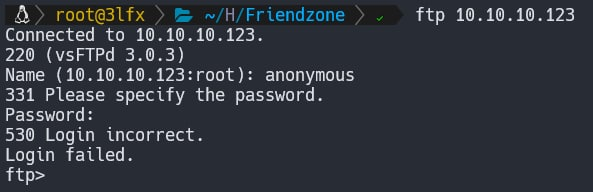
\includegraphics[width=0.99\textwidth]{informe4/imagenes/friendzone/02_ftp.png}
            \caption{Puerto ftp en Friendzone} 
        \end{figure}
        
        \large{Luego probamos con el puerto 'netbios ssn', usando la herramienta 'smbmap'.}
        \par
        \begin{figure}[H]
            \centering
            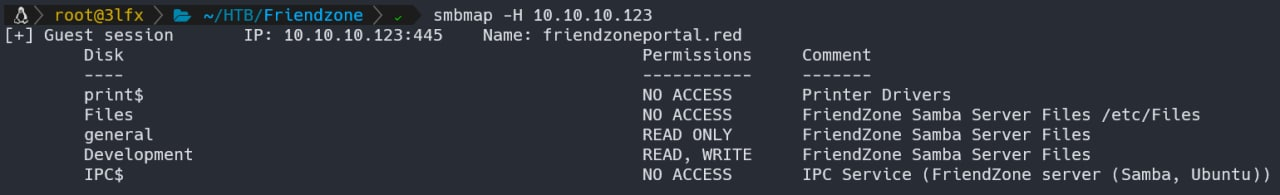
\includegraphics[width=0.99\textwidth]{informe4/imagenes/friendzone/03_smbmap.png}
            \caption{Hallazgo de la herramienta smbmap en Friendzone} 
        \end{figure}

        \large{Identificamos dos carpeta a las que se tiene acceso, una llamada genarl con acceso solo para leer y otra con nombre Development con accesos para leer y escribir. Revisamos la carpeta general.}
        \par
        \begin{figure}[H]
            \centering
            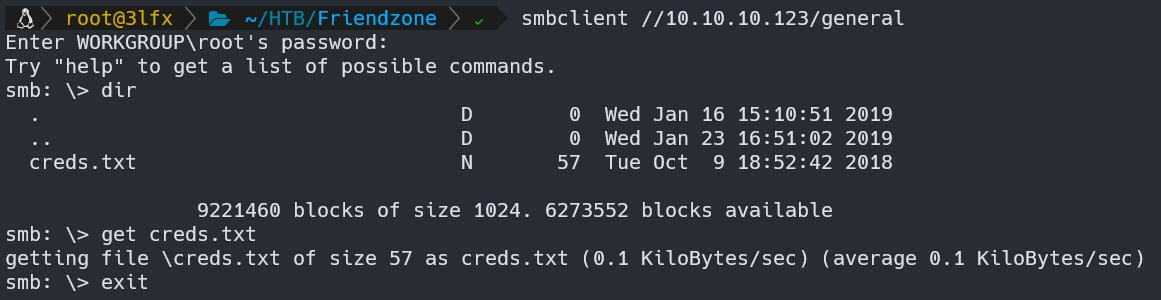
\includegraphics[width=0.99\textwidth]{informe4/imagenes/friendzone/04_smb_creds.png}
            \caption{Carpeta general en Friendzone} 
        \end{figure}

        \large{Dentro de la carpeta general encontramos una archivo '.txt' con el nombre creds, el cual parece una abreviacion de credenciales, por lo cual revisamos el archivo y al hacerlo encontramos las credenciales de admin.}
        \par
        \begin{figure}[H]
            \centering
            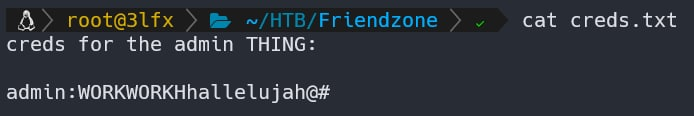
\includegraphics[width=0.99\textwidth]{informe4/imagenes/friendzone/05_cred_friendzone.png}
            \caption{Archivo creds.txt en Friendzone} 
        \end{figure}

        \begin{figure}[H]
            \centering
            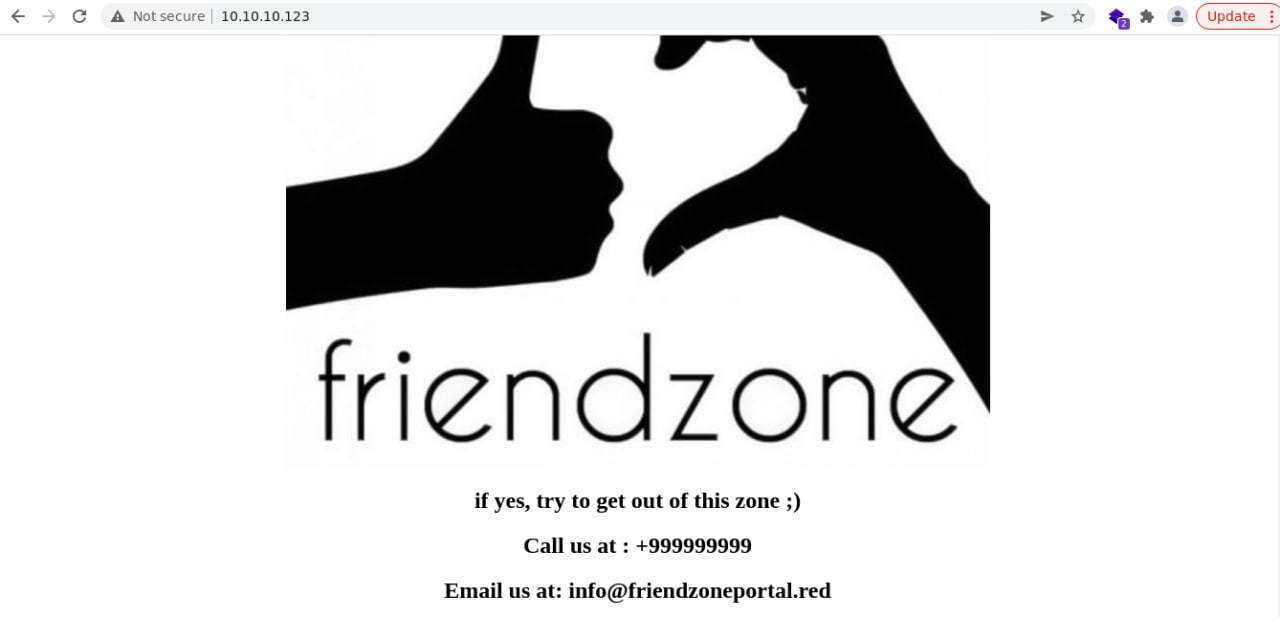
\includegraphics[width=0.99\textwidth]{informe4/imagenes/friendzone/06_web.png}
            \caption{Página web de la máquina Friendzone} 
        \end{figure}


    \subsubsection{Explotación}

    \subsubsection{Escalamiento de Privilegios}

    \subsubsection{Post-Explotación}

    \subsubsection{Recomendaciones de Mitigación}
